% DOCUMENT

\section{Equipo de trabajo}
\subsection{Procedimiento de estimación de recursos}
\par En este apartado se describe tanto el hardware, como el software y los recursos humanos que vamos a utilizar en la realización de este proyecto:
\par El hardware necesario se ha clasificado en:
\begin{itemize}[-]
\item \textbf{Entorno de desarrollo:} Para poder desarrollar correctamente el sistema, CARSAFETY nos proporcionará un automóvil sobre el que trabajaremos. Esto, al ser un coste asumido por el cliente no viene reflejado en el documento de costes. Para poder adaptar correctamente el proyecto a los vehículos de CARSAFETY, será necesario realizar un estudio exhaustivo para que no haya errores de adaptabilidad y sea completamente integrable.
\item \textbf{Entorno de producción:} Debido a que ya se ha realizado el estudio de viabilidad del sistema, el cliente se ha decantado por una de las alternativas que le propusimos, por lo que sabemos con exactitud qué elementos hardware son necesarios para la realización del proyecto. Es por ello que las cámaras, los sensores y otros elementos de computación necesarios se reflejarán en la partida de costes.
\end{itemize}
\par Para la realización de este proyecto se ha pensado utilizar herramientas para favorecer el trabajo en grupo, la coordinación y la comunicación entre los miembros del equipo. Casi todas estas herramientas necesitan una licencia para poder ser utilizadas, estando el precio reflejado en el documento de costes. Las herramintas que se utilizarán son las siguientes: Github, Office 365, Toggl, Trello, Slack, Google Apps for Work, Photoshop y Atom (Herramienta gratuita).
\par Los recursos humanos implicados en el proyecto estarán formados por siete personas, cada una teniendo asignada una tarea específica. El trabajo conjunto realizado por cada una de estas siete personas tendrá como resultado un buen desarrollo del proyecto adaptándose lo máximo posible a las necesidades del cliente.

\subsection{Equipo de trabajo}
\par El equipo de trabajo estará formado por los siguientes miembros:
\begin{itemize}
\item \textbf{Jefe de proyecto:} es la persona responsable de la gestión del proyecto. Se debe encargar de que el cliente se encuentre satisfecho durante todo momento con el proyecto que se está generando, cumpliendo con los costes y los plazos de entrega definidos. Al igual que el equipo de proyecto, el esfuerzo y trabajo del jefe de proyecto se verán recompensados económicamente.
  \begin{itemize}
  \item \textbf{Responsable:} Alberto García Hernández
  \end{itemize}
\item \textbf{Analista de sistemas:} es la persona encargada de elaborar los requisitos del sistema, de tal manera que se correspondan con las especificaciones establecidas por el cliente que solicita el sistema.
  \begin{itemize}
  \item \textbf{Responsable:} Daniel González de la Hera
  \end{itemize}
\item \textbf{Gestión de configuración:} es el responsable de asegurar que los cambios realizados en el sistema no afecten a la calidad del mismo durante cualquiera de las etapas de desarrollo. \begin{itemize}
  \begin{itemize}
  \item \textbf{Responsable:} Juan Abascal Sánchez
  \end{itemize}
\item \textbf{Gestión de calidad:} es el responsable de garantizar que el sistema sea consistente, además de definir los estándares de calidad para que el cliente esté satisfecho con el producto. \begin{itemize}
  \begin{itemize}
  \item \textbf{Responsable:} Adriana Lima
  \end{itemize}
\item \textbf{Responsable de pruebas:} es el responsable de definir las pruebas necesarias para asegurar que el producto satisface los requisitos establecidos, para tratar de reducir el número de fallos y limitaciones del sistema.
  \begin{itemize}
  \item \textbf{Responsable:} Carlos Olivares Sanchez-Manjavacas.
  \end{itemize}
\item \textbf{Desarrolladores:} es el equipo encargado de desarrollar los requisitos establecidos.
  \begin{itemize}
  \item \textbf{Responsables:} Carlos Tormo Sánchez y Irina Shayk.
  \end{itemize}
\end{itemize}

\subsection {Organigrama del equipo}
\par El organigrama del equipo de trabajo es plano con la excepción del jefe de proyecto, quien se sitúa en el puesto más alto del equipo. A continuación, se mostrará dicho organigrama:

\begin{figure}[H]
\begin{center}
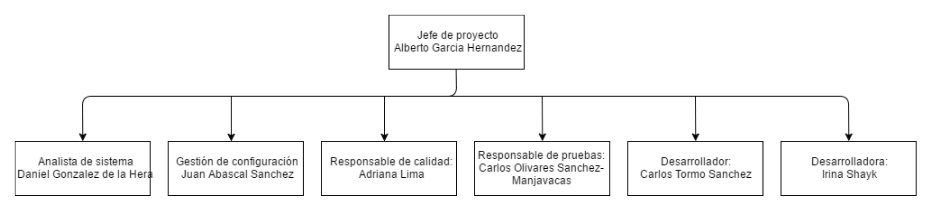
\includegraphics[width=0.8\textwidth]{./img/Org.png}
\end{center}
\caption{Organigrama del equipo}
\label{tab:horasTotales}
\end{figure}


\subsection {Organización de los trabajos}
\par En primer lugar, el jefe del proyecto y el analista de sistemas se reunirán con el cliente para identificar sus necesidades y obtener una primera versión de los requisitos que debe tener el sistema. Tras esta primera reunión, los analistas estudiarán los requisitos y determinarán si hay alguno que no encaje bien o no se pueda realizar. Una vez finalizado este estudio, volverá a haber una reunión con el cliente para hacer una valoración del estudio y especificar de manera correcta todos los requisitos. A parte de esta primera toma de contacto con el cliente, durante el desarrollo del proyecto habrá más reuniones ya que siempre surgen pequeños problemas o limitaciones que son necesarias comunicarle.
\par A continuación, el analista de sistemas y el equipo de desarrollo se reunirán para empezar a desarrollar el diseño de la aplicación y posteriormente su desarrollo. En este punto, el responsable de la gestión de configuración se tiene que asegurar que se cumple con las especificaciones dadas por el cliente. Además, el responsable de la gestión de calidad, tiene que asegurarse que durante toda esta fase se están cumpliendo los estándares de calidad definidos en el plan de calidad entregado al cliente.
\par Finalmente, el responsable de pruebas, a medida que los subsistemas encargados por el cliente estén disponibles, será el encargado de realizar las pruebas necesarias para poder entregarle al cliente un producto fiable, completo y eficiente.
\par En todo momento el jefe de proyecto irá supervisando cada una de las actividades para asegurarse que se cumple con la metodología definida, así como para asegurarse que se cumplen los plazos acordados con el cliente.
